\documentclass{standalone}

\usepackage{tikz}

\begin{document}
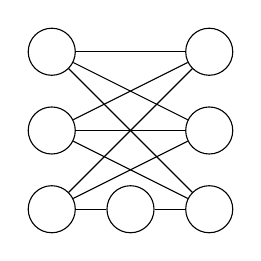
\begin{tikzpicture}
\tikzstyle{vertex}=[circle, draw, minimum size=17pt, inner sep=0pt]

\node[vertex] (A) at (0,0) {};
\node[vertex] (B) at (0,1) {};
\node[vertex] (C) at (0,2) {};
\node[vertex] (X) at (2,0) {};
\node[vertex] (Y) at (2,1) {};
\node[vertex] (Z) at (2,2) {};
\node[vertex] (v) at (1,0) {};

\path
(A) edge (Y)
    edge (Z)
(B) edge (X)
    edge (Y)
    edge (Z)
(C) edge (X)
    edge (Y)
    edge (Z)
(v) edge (X)
    edge (A);
\end{tikzpicture}
\end{document}

